\documentclass{article}
\usepackage{a4header,amsmath,amsthm}
\usepackage{amsmath,amsthm}
\usepackage{tikz}
\usetikzlibrary{calc,intersections}

\newcommand{\software}[1]{\textit{#1}}
\newcommand{\newterm}[1]{\textbf{#1}}
\newtheorem*{theorem}{Theorem}
\newtheorem*{definition}{Definition}
\newtheorem*{construction}{Construction}



\begin{document}
This document describes the construction of harmonic points in the
(Desarguesian) projective plane. The motivation is an exercise in learning to
use the LaTeX drawing software \software{tikz}


The construction makes use of Desargues' Theorem:
\begin{definition}
  Two triangles $ABC$ and $DEF$ are in perspective from a point if the
  lines   $AD,BE$ and  $CF$ joining corresponding vertices are concurrent.  \\
  Two triangles $ABC$ and $DEF$ are in perspective from a line if the points
  of intersection of corresponding sides $AB \cdot DE, BC \cdot EF $ and
  $AC \cdot DF$ are co-linear. 
\end{definition}
\begin{theorem}[Desagues]
  If two triangles $ABC$ and $DEF$ are in perspective from a point they are in perspective from a line.\\
  Dually:\\
  If two triangles $ABC$ and $DEF$ are in perspective from a line they are in perspective from a point.
\end{theorem}
\begin{definition}
  Four lines in a projective plane with their six points of intersection form a \newterm{complete quadrilateral}.
\end{definition}

\begin{tikzpicture}[
    ppoint/.style={circle, draw,fill,inner sep = 1pt }]
  
   \node (p12) at (2,3)[ppoint, label=right:$p_{12}$] {};
   \node (p14) at (1,1)[ppoint,label=95:$p_{14}$] {};
   \node (p24) at (0,-1)[ppoint,label=175:$p_{24}$] {};
   \draw (2.5,4) --  (-0.5,-2);
   \node (p23) at (4,1)[ppoint,label=above:$p_{23}$] {};
   \node (p13) at (4.5,0.5)[ppoint,label=85:$p_{13}$] {};
   \node[ppoint] (p34) at (3.3333,0.6666)[label=above:$p_{34}$] {};
 
   \draw (1,4) -- (5.5,-0.5);
   \draw (0.3,1.1) -- (5.2,0.4);
   \draw (-2,-2) -- (6,2);
\end{tikzpicture}
%\pagebreak
\begin{definition}
  The three lines joining the pairs of point not ona commom line form the \newterm{diagonals} of the complete quadrilatal.
\end{definition}
\begin{figure}
  \caption{Diagram draw using explicitly calculated end points.}

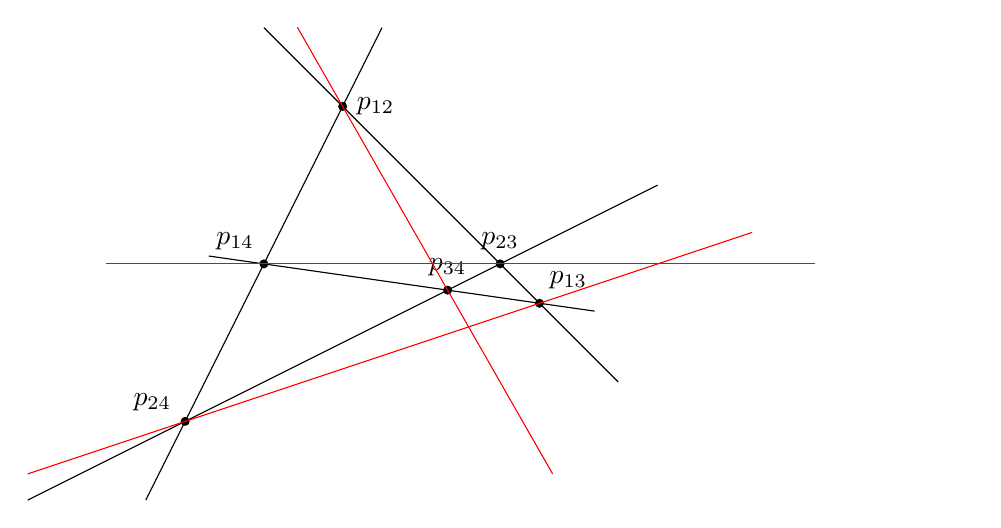
\begin{tikzpicture}
  [ppoint/.style={circle, draw,fill,inner sep = 1pt }]
  \clip (-2,-2) rectangle (10,4);
   \node[ppoint] (p12) at (2,3)[label=right:$p_{12}$] {};
   \node[ppoint] (p14) at (1,1)[label=95:$p_{14}$] {};
   \node[ppoint] (p24) at (0,-1)[label=175:$p_{24}$] {};
   \draw[ppoint] (2.5,4) --  (-0.5,-2);
   \node[ppoint] (p23) at (4,1)            [label=above:$p_{23}$] {};
   \node[ppoint] (p13) at (4.5,0.5)        [label=85:$p_{13}$] {};
   \node[ppoint] (p34) at (3.3333,0.6666)  [label=above:$p_{34}$] {};
 
   \draw (1,4) -- (5.5,-0.5);
   \draw (0.3,1.1) -- (5.2,0.4);
   \draw (-2,-2) -- (6,2);
   % The diagonals
   \begin{scope}
     \draw[red] (-1,1) -- (8,1);
     \draw[red] (0.6666,5.3333) -- (4.6666,-1.66666);
     \draw[red] (-2.7,-1.9) -- (7.2,1.4);
   \end{scope}
\end{tikzpicture}
\end{figure}

The code above created by explicitly calculating end points  of lines.

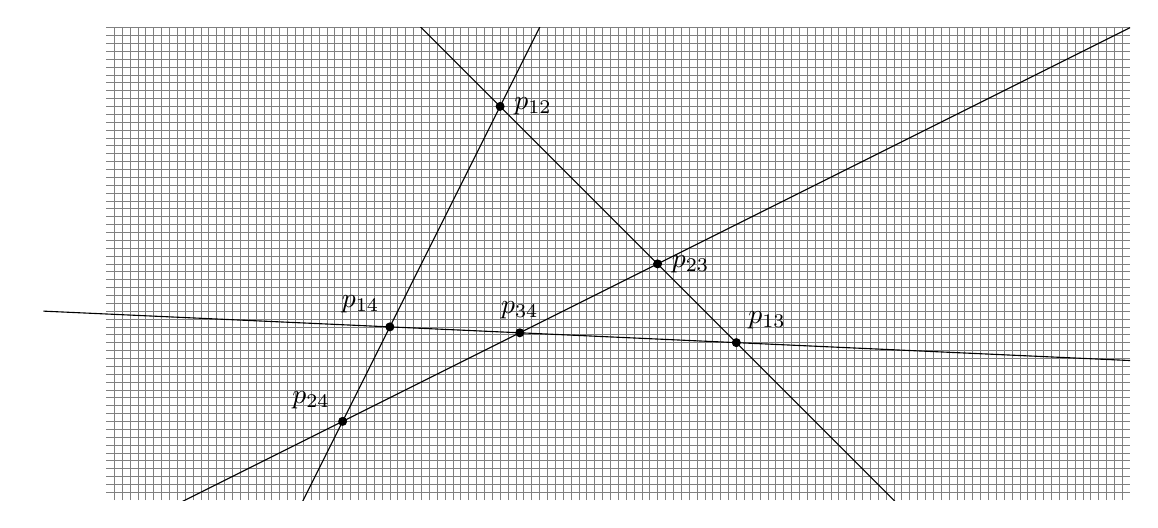
\begin{tikzpicture}
  [ppoint/.style={circle, draw,fill,inner sep = 1pt }]
  \clip (-4,-2) rectangle (10,4);
% Temporary coordinate grid
  \draw[step=0.1,gray, very thin] (-3,-2)grid(10,4);
  % Define point postions using \coordinate
  \coordinate (p12) at (2,3);
  \coordinate (p24) at (0,-1);
  \coordinate (p23) at (4,1);
  \coordinate (p14) at ($0.3*(p12)+0.7*(p24)$);
  \coordinate (p13) at ($-0.5*(p12)+1.5*(p23)$);
  % Calculate end points for lines.
  \coordinate (d3) at ($(p24)-(p12)$);
  \coordinate (b3) at ($(p12)-(d3)$);
  \coordinate (e3) at ($(p24)+(d3)$);

  \coordinate (d4) at ($(p23)-(p12)$);
  \coordinate (b4) at ($(p12)-(d4)$);
  \coordinate (e4) at ($(p23)+2*(d4)$);

  \coordinate (d1) at ($(p23)-(p24)$);
  \coordinate (b1) at ($(p24)-(d1)$);
  \coordinate (e1) at ($(p23)+3*(d1)$);

  \coordinate (d2) at ($(p13)-(p14)$);
  \coordinate (b2) at ($(p14)-(d2)$);
  \coordinate (e2) at ($(p13)+3*(d2)$);
 
  %Name the lines
  \path[name path = l1] (p23) -- (p24);
  \path[name path = l2] (p13) -- (p14);
  \path[name path = l3] (p12) -- (p24);
  \path[name path = l4] (p12) -- (p23);
  % Use the intersection software to define p34
  \path[name intersections={of=l1 and l2, by= p34}];
  %draw the lines 
  \draw (b3) -- (e3);
  \draw (b4) -- (e4);
  \draw (b1) -- (e1);
  \draw (b2) -- (e2);
% Show and label the points of intersection.
  \node at (p12)[ppoint, label=right:$p_{12}$] {};
  \node at (p24)[ppoint, label=135:$p_{24}$] {};
  \node at (p23)[ppoint, label=right:$p_{23}$] {};
  \node at (p14)[ppoint, label=100:$p_{14}$] {};
  \node at (p13)[ppoint, label=60:$p_{13}$] {};
  \node at (p34)[ppoint, label=above:$p_{34}$] {};
\end{tikzpicture}

%\pagebreak

There are three pairs of points $p_{14}, p_{23}$, $p{12}, p_{34}$ and $p_{24},p_{13}$ that are not on a commom line. 
The lines through these points are referred to as the \newterm{diagonals}. Together they form the 
\newterm{diagonal point triangle}.

\begin{figure}
  
  \caption{Diagonal Point Triangle of a Complete Quadrangle}
 
  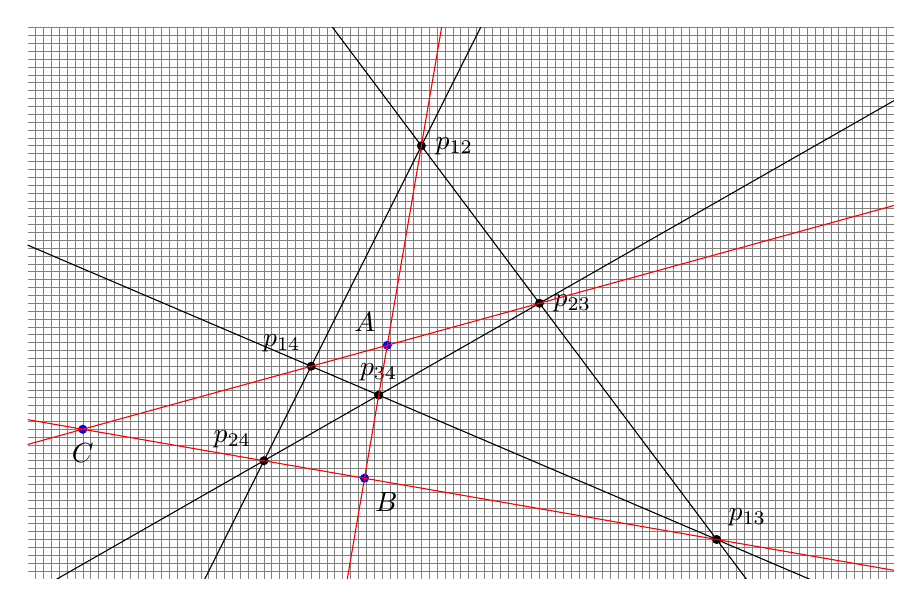
\begin{tikzpicture}
   [ppoint/.style={circle, draw,fill,inner sep = 1pt }]
    \clip (-3,-2.5) rectangle (8,4.5);
    % Temporary coordinate grid
    \draw[step=0.1,gray, very thin] (-3,-2.5)grid(10,4.5);
    % Define intersection point positions using \coordinate
    \coordinate (p12) at (2,3);
    \coordinate (p24) at (0,-1);
    \coordinate (p23) at (3.5,1.0);
    \coordinate (p14) at ($0.3*(p12)+0.7*(p24)$);
    \coordinate (p13) at ($-1.5*(p12)+2.5*(p23)$);
   
    % Calculate end points for lines.
    \coordinate (d3) at ($(p24)-(p12)$);
    \coordinate (b3) at ($(p12)-(d3)$);
    \coordinate (e3) at ($(p24)+(d3)$);
    
    \coordinate (d4) at ($(p23)-(p12)$);
    \coordinate (b4) at ($(p12)-(d4)$);
    \coordinate (e4) at ($(p23)+2*(d4)$);
    
    \coordinate (d1) at ($(p23)-(p24)$);
    \coordinate (b1) at ($(p24)-(d1)$);
    \coordinate (e1) at ($(p23)+3*(d1)$);
    
    \coordinate (d2) at ($(p13)-(p14)$);
    \coordinate (b2) at ($(p14)-(d2)$);
    \coordinate (e2) at ($(p13)+3*(d2)$);
    
    
    %Name the lines
    \path[name path = l1] (p23) -- (p24);
    \path[name path = l2] (p13) -- (p14);
    \path[name path = l3] (p12) -- (p24);
    \path[name path = l4] (p12) -- (p23);
    
    % Use the intersections software to define p34
    \path[name intersections={of=l1 and l2, by= p34}];
    
    %draw the lines 
    \draw (b3) -- (e3);
    \draw (b4) -- (e4);
    \draw (b1) -- (e1);
    \draw (b2) -- (e2);
    % Show and label the points of intersection.
    \node at (p12)[ppoint, label=right:$p_{12}$] {};
    \node at (p24)[ppoint, label=135:$p_{24}$] {};
    \node at (p23)[ppoint, label=right:$p_{23}$] {};
    \node at (p14)[ppoint, label=100:$p_{14}$] {};
    \node at (p13)[ppoint, label=60:$p_{13}$] {};
    \node at (p34)[ppoint, label=above:$p_{34}$] {};
    
    % Draw the diagonals
    
    % Define  suitable end points for the diagonals
    \coordinate (D1) at ($(p12)-(p34)$);
    \coordinate (B1) at ($(p34)-(D1)$);
    \coordinate (E1) at ($(p12)+(D1)$);
    
    \coordinate (D2) at ($(p14)-(p23)$);
    \coordinate (B2) at ($(p23)-3*(D2)$);
    \coordinate (E2) at ($(p14)+2*(D2)$);
    
    \coordinate (D3) at ($(p24)-(p13)$);
    \coordinate (B3) at ($(p13)-(D3)$);
    \coordinate (E3) at ($(p24)+(D3)$);
    
    \path[name path = DL1] (B1) -- (E1);
    \path[name path = DL2] (B2) -- (E2);
    \path[name path = DL3] (B3) -- (E3);
    
    \path[name intersections={of=DL1 and DL2, by= A}];
    \path[name intersections={of=DL3 and DL1, by= B}];
    \path[name intersections={of=DL2 and DL3, by= C}];

    \node[blue] at (A)[ppoint, label=120:$A$] {};  
    \node[blue] at (B)[ppoint, label=280:$B$] {};  
    \node[blue] at (C)[ppoint, label=below:$C$] {};  
    
    \draw[red]  (B1)-- (E1);
    \draw[red]  (B2)-- (E2);
    \draw[red]  (B3)-- (E3);
  \end{tikzpicture}
\end{figure}

There are four points on  each line of the quadrilateral. These points are said to be in \newterm{harmonic range}.

\begin{theorem}
  Given points A and B with a third point C on the line AB there is a unique point D the \newterm{harmonic conjugate}~of C so that
ABCD form an harmonic range.
\end{theorem}
\begin{construction}
  Choose a point $F$ not on the line $ABC$ and a point $H$ on CF.

  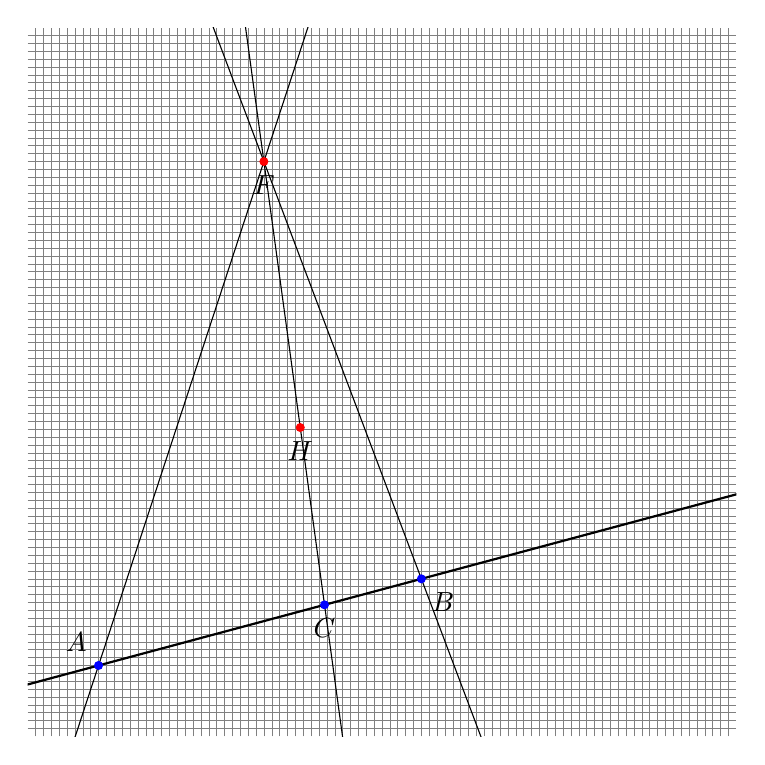
\begin{tikzpicture}
    [ppoint/.style={circle, draw,fill,inner sep = 1pt }]
    \clip (-1,-1) rectangle (8,8);
    % Temporary coordinate grid
    \draw[step=0.1,gray, very thin] (-1,-1)grid(8,8);
    % Define intersection point positions using \coordinate
    \coordinate (cA) at (-0.1,-0.1);
    \coordinate (cB) at (4,1);
    \coordinate (cC) at ($0.3*(cA)+0.7*(cB)$);
    \coordinate (cF) at (2,6.3);
    \coordinate (cH) at ($0.6*(cC)+0.4*(cF)$);
  %%  % \coordinate (p13) at ($-1.5*(p12)+2.5*(p23)$);
   
    % calculate end points for lines.
    \coordinate (DL) at ($(cB)-(cA)$);
    \coordinate (LB) at ($(cA)-(DL)$);
    \coordinate (LE) at ($(cB)+(DL)$);
    
    \coordinate (cD1) at ($(cF)-(cC)$);
    \coordinate (cB1) at ($(cC)-(cD1)$);
    \coordinate (cE1) at ($(cF)+2*(cD1)$);
    
    \coordinate (cD2) at ($(cF)-(cA)$);
    \coordinate (cB2) at ($(cA)-(cD2)$);
    \coordinate (cE2) at ($(cF)+3*(cD2)$);
    
    \coordinate (cD3) at ($(cF)-(cB)$);
    \coordinate (cB3) at ($(cB)-(cD3)$);
    \coordinate (cE3) at ($(cF)+(cD3)$);
   
    %Draw the lines 
    \draw[thick]  (LB)--(LE);
    \draw  (cB1) -- (cE1);
    \draw  (cB2) -- (cE2);
    \draw  (cB3) -- (cE3);

    \node[blue] at (cA)[ppoint, label=120:$A$] {};  
    \node[blue] at (cB)[ppoint, label=280:$B$] {};  
    \node[blue] at (cC)[ppoint, label=below:$C$] {};  
    \node[red] at (cF)[ppoint, label=below:$F$] {};  
    \node[red] at (cH)[ppoint, label=below:$H$] {};  
    

  \end{tikzpicture}
\end{construction}

\end{document}
%%% Local Variables: 
%%% mode: latex
%%% TeX-master: t
%%% End: 
